%% use article style

\documentclass[12pt]{article}
\usepackage{amsmath,amssymb,amsthm,amsfonts}
\usepackage{graphicx}
\title{A new look at Pompeiu Triangles}
\begin{document}
\maketitle
\section{Introduction}
Ptolemey's theorem states that if $ABCD$ is a cyclic quadrilateral, then $AB\cdot CD+BC\cdot DA=AC\cdot BD$. When $D$ does not belong to the circumcircle of $ABC$, then the following inequality holds: $AB\cdot CD+BC\cdot DA>AC\cdot BD$. If $ABC$ is an equilateral triangle (and using $P$ instead of $D$ to denote the fourth point), then $PC+PA \geq PB$. This is because $AB=BC=CA$ and $P$ does not belong to the circumcircle of $ABC$. Given that the inequality above (called the triangle inequality) holds, one can construct a triangle with sides $PA$, $PB$ and $PC$.  Such a triangle is called a Pompeiu triangle. The name comes from the Romanian mathematician Dimitrie Pompeiu, who studied these triangles in 1929. An interesting property of Pompeiu triangles is that their areas can be calculated using elementary geometry. Moreover, their areas are related to other geometric properties. In this paper, we will present a new way of deriving the formula to 
calculate the area of a Pompeiu triangle. The derivation involves circular inversions. We also derive a formula to relate this area to the distance of point D to the circumcircle of $ABC$. A derivation based on inversions was presented by Benyi and Casu (2009). However, the derivation presented here is simpler and more elegant. 

\section{Circular inversions}
Inversions are a powerful tool in geometry. They are used to prove many theorems. In this section, we will present the basic properties of inversions. We will also present a formula to calculate the area of a triangle using inversions.

In plane geometry the inverse of a point $P$ with respect to a reference circle with center $O$ and radius $k$ is a point $P'$, lying on the ray from $O$ through $P$ such that

\begin{equation}
OP\cdot OP'=k^2
\label{eq:inversion}
\end{equation}

A remarkable property of inversions is that they transform circles that go through the center of inversion into straight lines. This is a property that we will use in this paper to derive the formula for the area of a Pompeiu triangle. For a proof of this property, see https://artofproblemsolving.com/wiki/
index.php/Circular\_Inversion.
Another property that we will use is that if $A'$ and $B'$ are the inverses of points $A$ and $B$ then 

\begin{equation}
{A'B'}={AB}\frac{k^2}{OA\cdot OB}
\label{eq:inversion2}
\end{equation}

\section{The area of a Pompeiu triangle}

%% insert figure 1 here
For a given equilateral triangle $\Delta ABC$, we can apply an inversion with respect to a reference circle with center $A$ and radius $k$, and transform points $A$ and $B$ into point $A'$ and $B'$. A point $P$ interior to triangle $\Delta ABC$ is transformed into $P'$, which is exterior to triangle $\Delta AB'C'$. This is illustrated in Figure \ref{fig:pompeiuTriangles1}. It may be noticed in this figure that the area of $\Delta B'P'C'$ can be determined from the areas of triangles $\Delta AB'P'$, $\Delta AP'C'$ and $\Delta AB'C'$.  More specifically, if we denote the area of any given triangle $\Delta ABC$ by $S(ABC)$, then

\begin{equation}
S(B'P'C')=S(AB'P')+S(AP'C')-S(AB'C')
\label{eq:area1}
\end{equation}

To relate equation ref{eq:area1} to the area of a Pompeiu triangle, we need to express the areas of triangles $\Delta B'P'C'$, $\Delta AB'P'$, $\Delta AP'C'$ and $\Delta AB'C'$ in terms of the untransformed distances among points $A$,$B$,$C$ and $P$.

According to equation \ref{eq:inversion2}, $B'C'=BC\frac{k^2}{AB\cdot AC}$, $B'P'=BP\frac{k^2}{AB\cdot AP}$ and $P'C'=PC\frac{k^2}{AP\cdot AC}$. 
However, $AB$=$BC$=$AC$=$a$. Therefore, $B'C'=\frac{k^2}{a}$, $B'P'=BP\frac{k^2}{a\cdot AP}$ and $P'C'=PC\frac{k^2}{a\cdot AP}$. Rewriting $B'C'$ as $B'C'=PA \frac{k^2}{a \cdot AP}$, we can notice that the sides of triangle $\Delta B'P'C'$ are proportional to the sides of triangle formed with segments $PA$, $PB$, $PC$. The scale factor is $\frac{k^2}{a \cdot AP}$. Therefore, the area of $\Delta B'P'C'$ is proportional to the area of Pompeiu triangle $(PA,PB,PC)$. More specifically, $S(B'P'C')=S(P(PA,PB,PC))(\frac{k^2}{a PA})^2$.

\begin{figure}[h]
\centering
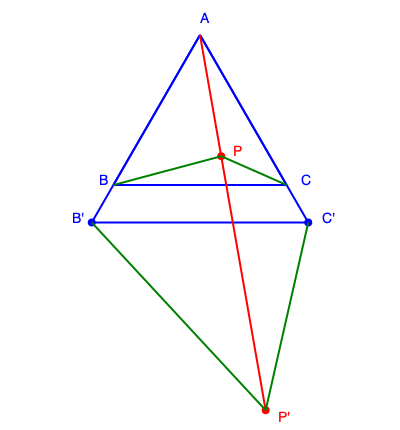
\includegraphics[width=0.5\textwidth]{pompeiuTriangle.png}
\caption{A Pompeiu triangle}
\label{fig:pompeiuTriangles1}
\end{figure}

To express the area of triangles $\Delta AB'P'$ as a function of $S(ABP)$, we can use $S(AB'P')=\frac {AB'\cdot AP' \cdot \sin(B'AP')}{2}$=
$\frac{1}{2} \cdot \frac {k^2} {AB} \cdot \frac {k^2}{AP} \cdot \sin(BAP)$=$\frac {k^4} {AB^2 PA^2} \cdot \frac {AB \cdot AP \cdot \sin(BAP)} {2}$=$\frac {k^4}{a^2 PA^2} S(ABP)$. Similarly, $S(AP'C')=\frac {k^4}{a^2 PC^2} S(APC)$. 
\end{document}